\documentclass[book.tex]{subfiles}
\begin{document}
\label{chapter_software_architecture}
\section{About the source code}
The source code for Commander Keen Episodes 1--5 is unavailable, as the current owner Zenimax\footnote{June 24, 2009, id Software was acquired by ZeniMax Media (owner of Bethesda Softworks).} has shown no interest at the time of writing in selling the intellectual property. Fortunately, the ownership of Commander Keen in Keen Dreams was in the hands of Softdisk. In June 2013, developer Super Fighter Team licensed the game from Flat Rock Software, the owners of Softdisk at the time, and released a version for Android devices.\\

\par
The following September, an Indiegogo crowdfunding campaign was launched to purchase the rights from Flat Rock for US\$1500 in order to release the game's source code and publish it on multiple platforms. The campaign did not reach the goal, but its creator Javier Chavez made up the difference, and the source code was released under GNU GPL-2.0-or-later soon after.


\section{Getting the source code}
\label{section:source_code}
The source code is available on GitHub. It is essential to use the source code from shareware version 1.13, otherwise you may encounter compatibility issues due to incompatible map and graphics headers\footnote{See issue \#7 on https://github.com/keendreams/keen.}. To get the correct source code, run the following commands in the console \\

\par
\tcode{keen13_github.txt}\\

\section{Exploring the source code}
After downloading the repository from GitHub, a folder named 'keen' is created, containing all the source files. The \cw{cloc.pl} tool can be used to analyze the folder and generate statistics about the source code. This tool is useful for getting an idea of what to expect.\\

\par
\begin{minipage}{\textwidth}
\lstinputlisting[]{code/cloc.txt}
\end{minipage}

\vspace{8pt}
\par
Approximately 85\% of the code is in C, with assembly used for performance-critical optimizations and low-level I/O operations such as video and audio handling. \\

\par
Source lines of code (SLOC) is helpful for understanding the relative size of the codebase compared to modern software. For instance, Inkscape (a vector graphics editor tool I used to create the drawings in this book) has 544,508 SLOC, Unreal Engine 4 has 2,300,000 SLOC and Microsoft Office 2013 is estimated to have 45,000,000 SLOC. This illustrates how small Commander Keen is compared to modern software codebases.\\

\trivia{The game \textit{Red Dead Redemption II} is estimated to have 60 million SLOC, the highest amount for a game at the time of writing this book.}\\

 
\par 
Besides the source code, the repository also contains two folders featuring:
\begin{itemize}
\item A \cw{static} folder with header and dictionary files for loading assets and maps, and a tool \cw{makeobj.c} to convert these files into OBJ-files (this is explained in the next section).
\item An \cw{lscr} folder for loading and decompressing Softdisk text files.
\end{itemize}

\section{Compiling source code}
Now let's compile the source code. To compile the code like it's 1990, you need the following software:
\begin{itemize}
\item Commander Keen source code.
\item DOSBox.
\item Borland C++ 3.1.
\item Commander Keen: Keen Dreams 1.13 shareware (for the assets).
\end{itemize}

\par
After setting up DOSBox and installing Borland C++ 3.1\footnote{You can find a complete tutorial in "Let's compile like it's 1992" on fabiensanglard.net}, download the source code from GitHub. Once DOSBox is running and you have navigated to the \cw{keen} folder, create a folder to store your compiled object files. \\

\par
\tcode{mkdir.txt}\\
\par
The \cw{static} folder contains the Huffman dictionaries (\cw{DICT}) and headers (\cw{HEAD}) from the generated graphics, sound and map assets, stored as raw game data files. The team created a special tool called \cw{makeobj} that takes these data files and wraps them into DOS-compatible \cw{.OBJ} files, so that a C compiler (such as Borland C++) can link them directly into the game's executable. The tool creates a "symbol" within the object file so that the game's source code can access the embedded data just like any other global variable. \\

\par
\tcode{makeobj.txt}\\

\par
To generate all static \cw{OBJ} header files, simply enter the following command:\\
\par
\tcode{static.txt}\\

\par
After that, return to the \cw{keen} folder and open Borland C++. Open the \cw{kdreams.prj} project file. Before compiling, adjust the directory settings by selecting Options -> Directories and change the values as shown on the next page. \\

\par
Now it's time to compile. Go to Compile -> Build All, and voil\`a! The game executable is stored in the \textbackslash{}OBJ folder. The final step is to copy \cw{kdreams.exe} into the Keen shareware folder. You can now play your compiled version of \textit{Commander Keen}. \\

\begin{figure}[H]
\centering
  \fbox{\includegraphics[width=1.0\textwidth]{screenshots_300dpi/borland_directories.png}}
\end{figure}

 \begin{figure}[H]
\centering
  \fbox{\includegraphics[width=1.0\textwidth]{screenshots_300dpi/borland_compile.png}}
  \caption{Compiling Commander Keen in Borland C++ 3.1.}
\end{figure}

\section{Executable compression}
Checking the size of the compiled program, we see\\
\par
\tcode{source_compile_size.txt}\\

\par
As mentioned earlier, Softdisk did not allow distribution of games larger than 360 KiB. The compiled executable alone already occupies 349 KiB, and it still needed to accommodate graphics, map, and audio assets. With only 11 KiB remaining, the team needed a way to compress the executable to ensure everything would fit on one floppy disk.\\

\par
To compress the executable, the team used a small utility called LZEXE. It was one of the first widely used executable file compression tools for DOS computers. LZEXE allowed DOS executables to be launched without requiring an explicit decompression step. Most other compression or packing utilities required an additional step (and often additional disk space) to accomplish this.\\


\par
\begin{fancyquotes}
I wrote LZEXE in 1989 and 1990 when I was 17. At that time, hard disks were small and expensive, and 5\nicefrac{1}{4}-inch floppies were small (360KiB). Since I had only two floppy drives on my PC (an Amstrad PC1512), saving space was really an issue.\\

\par
Although I wrote LZEXE for my own use, I gave it to some friends, and it was then put on some BBS’s. LZEXE became then very famous, although I did not do anything to promote it. This success was quite unexpected for me.\\

\par
\textbf{Fabrice Bellard, LZEXE creator\protect\footnotemark}
\end{fancyquotes}\\
\addtocounter{footnote}{-1}
\stepcounter{footnote}
\footnotetext{See homepage of Fabrice Bellard: https://bellard.org/lzexe/.}


\par
The compression engine was built around the Lempel–Ziv–Storer–Szymanski (LZSS) algorithm, and the decompressor was designed to operate without using more memory than the final decompressed program required. This was more difficult than it might seem at first, because the tool had to ensure that there was never a moment when decompressed data overwrote an unread portion of the compressed data.\\

\par
An LZEXE-compressed program is a standard DOS executable, loaded in the standard way without any special trickery. Each executable file contains an EXE header, which specifies the initial layout of the executable in memory. One of its tasks is to initialize the stack, which is set up to a high area of uninitialized memory.\\

\par
The first task performed by the program is to move itself, including the decompression code and relocation table. This step is necessary because, if the compressed payload were decompressed in the same location where DOS originally loaded it, the decompressor would begin writing decompressed program data faster than it could read the compressed data, destroying its own source material.\\

\par
\begin{figure}[H]
\centering
 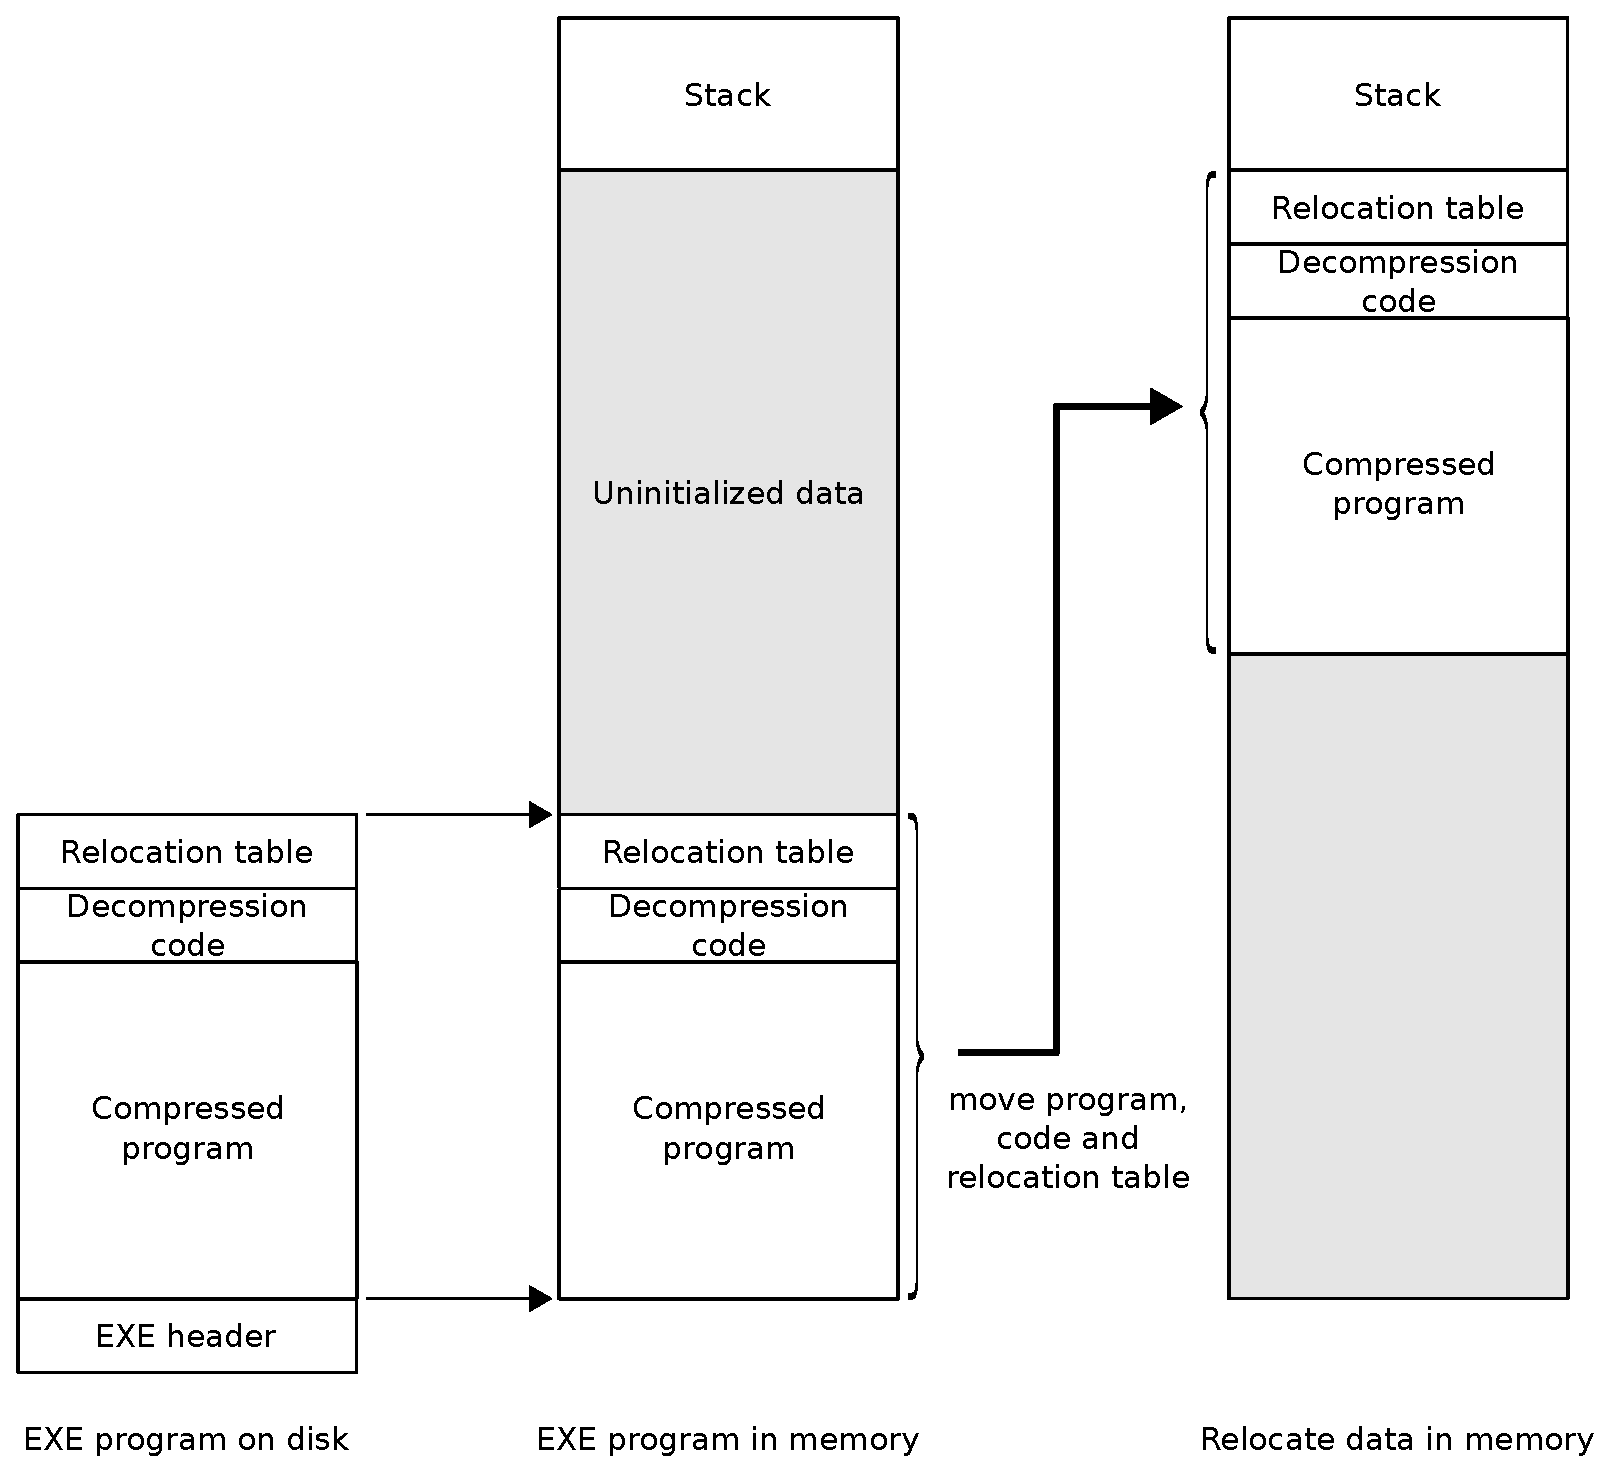
\includegraphics[width=1.0\textwidth]{imgs/drawings/LZ_decompresss_1.eps}
 \caption{Loading and relocating EXE program in memory (simplified).}
 \end{figure}

\par
Once relocated, the decompression code begins reading the compressed program and decompresses it back into the program’s original starting address. The heart of the decompressor is the LZSS algorithm, which operates by replacing repeated occurrences of data with references to earlier instances of that same data in the decompressed output\footnote{See https://cosmodoc.org/topics/lzexe/ for a detailed explanation of LZSS compression.}.

\par
\begin{figure}[H]
\centering
 \includegraphics[width=0.7\textwidth]{imgs/drawings/LZ_decompresss_2.eps}
 \caption{Decompression and final result in memory.}
 \end{figure}
 
\par
After the entire program has been decompressed, special attention is required for \cw{JMP} (jump) and \cw{CALL} instructions. Normal program execution is linear, with each instruction directly following the previous one. Jump and call instructions interrupt this flow and force the program to branch to arbitrary absolute addresses in the code.
However, under DOS there are no guarantees about the memory address at which an executable will be loaded. Depending on DOS itself, device drivers, reserved memory regions, and other factors, this address can — and frequently does — change from run to run. \\



\par
To solve this problem, DOS uses a relocation table. 
When an EXE file is created, all absolute addresses in the code are calculated under the assumption that the program will be loaded at address \cw{0000:0000h}, the absolute beginning of memory. The relocation table contains a list of locations within the executable where such absolute addresses appear. The DOS loader iterates through this table and patches each address \circled{1} by adding the program’s actual load address \circled{2}.\\

\vspace{-4pt}
\par
\begin{figure}[H]
\centering
 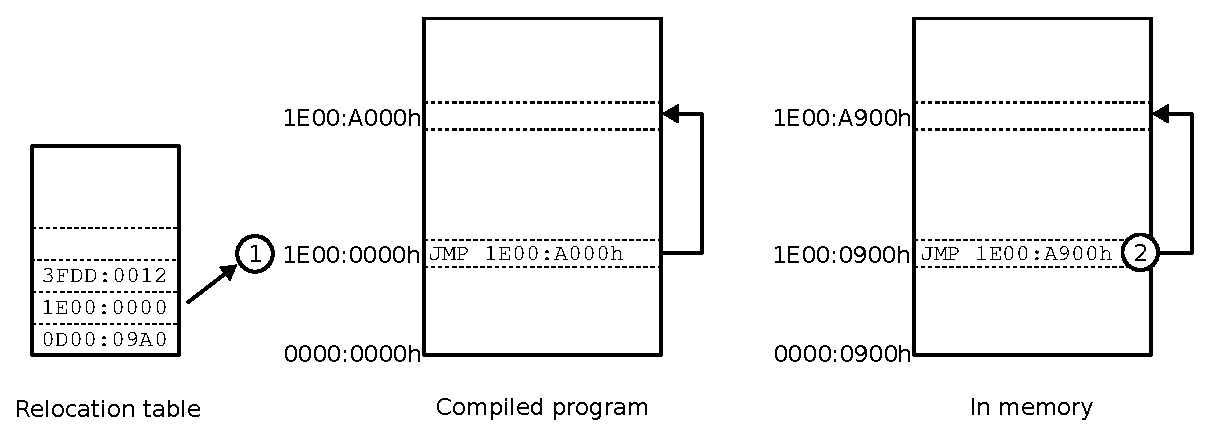
\includegraphics[width=1.0\textwidth]{imgs/drawings/relocation_table.eps}
 \caption{DOS relocation table.}
 \end{figure}

\par
DOS stores each relocation table entry as a 4-byte segment:offset pointer. This takes up quite a bit of space, since an average game has over 1,300 relocation table entries, which would occupy well over 5 KiB of space using the DOS scheme. LZEXE, by contrast, encodes only the distance from the previous fixup. This results in a far more efficient format, where most relocations require only a single byte. In practice, an LZEXE-compressed relocation table can be one-quarter the size of the equivalent DOS relocation table.\\




\par
At this point, memory contains exactly what it would have contained if the executable had never been compressed with LZEXE in the first place. And that’s how it all worked — everything happening in the split second between the user pressing the Enter key at the DOS prompt and the screen clearing to launch the game. The executable file is ultimately compressed to 80 KiB, achieving a 77\% reduction in file size.\\

\par
\begin{fancyquotes}
When I was trying to fit all the data for Keen 2 and Keen 3 on a 360K floppy and all the files wouldn't fit, I had to convert a bunch of files to .OBJ files (using a utility I developed), change the code to forgo the loading process for those files, then I had to link them into the KEEN EXE file, then finally I had to LZEXE the EXE file so it was much smaller.\\ 
\par
-- that was the only way that Keen 2 and 3 would fit on a 360K floppy.\\

\par
\textbf{John Romero\protect\footnotemark}
\end{fancyquotes}\\
\addtocounter{footnote}{-1}
\stepcounter{footnote}
\footnotetext{History of Commander Keen on https://legacy.3drealms.com/keenhistory.}


\pagebreak
\section{Main overview}
The game engine is divided into three blocks: 
\begin{itemize}
\item Control panel, which lets players configure and start the game.
\item 2D game engine, where players spend most of their time.
\item Sound system, which runs concurrently with either the control panel or 2D engine. 
\end{itemize}
The 2D engine communicates with the sound engine via function calls. The 2D engine sends sound requests to the sound engine, which processes them in its main loop. The sound engine controls the game’s heartbeat. It updates the global \cw{TimeCount} variable, which is used to time-control the game flow and screen refresh.\\

\par
\begin{figure}[H]
\centering
 \includegraphics[width=0.95\textwidth]{imgs/drawings/three_systems.eps}
 \caption{Game engine three main systems.}
 \end{figure}
 \par
 
\subsection{Unrolled Loop}
The first programmer-defined function that runs in any C program is named \cw{main()}, which resides in \cw{kd\_main.c}. When started with the \cw{/?} argument, the program displays an overview of available configuration parameters, such as  disabling sound cards or mouse. The control panel and 2D engine follow regular loops, but due to limitations explained later, the sound system is interrupt-driven and therefore operates outside the main loop. \\

\par
The first action taken by the program is to set the text color to light grey and the background to black, followed by game initialization, after which the main loop begins. \\
\par
\begin{minipage}{\textwidth}
\lstinputlisting[language=C]{code/unrolled_loop_main.c}
\end{minipage}
\par

\par
In \cw{InitGame()}, the program checks whether there is enough memory and brings up all the managers. Next, it loads all sounds and frequently used graphics (e.g. font and Commander Keen sprites) into memory.\\
\par
\begin{minipage}{\textwidth}
\lstinputlisting[language=C]{code/unrolled_loop_init.c}
\end{minipage}
\par
Then comes the core loop, where the menu and 2D engine are called forever.\\

\begin{minipage}{\textwidth}
\lstinputlisting[language=C]{code/unrolled_loop_demoloop.c}
\end{minipage}
\par
\cw{PlayLoop} contains the 2D engine. It is pretty standard with getting input, updating the state machine, scrolling, and refreshing the screen.\\

\par
\begin{minipage}{\textwidth}
\lstinputlisting[language=C]{code/unrolled_loop_playloop.c}
\end{minipage} 
\par
 
The interrupt system is started via the Sound Manager in \cw{SDL\_SetIntsPerSec(rate)}. The reason for interrupts is extensively explained in Chapter \ref{audio_and_heartbeat} "\nameref{audio_and_heartbeat}". In short, with DOS supporting neither processes nor threads, it was the only way to have something executed concurrently with the rest of the engine.


\section{Architecture}

The source code is structured in two layers. The ID\_* files are sub-systems called managers interacting with the hardware. These ID\_* managers were generic and reused in other id Software games (e.g. \textit{Hovertank One}, \textit{Catacomb 3-D} and \textit{Wolfenstein 3D}). The KD\_* files were written specifically for Commander Keen.
\par
\begin{figure}[H]
\centering
\includegraphics[width=\textwidth]{imgs/drawings/layers.eps} 
\caption{Commander Keen source code layers.}
 \end{figure}
 \par
There are six managers in total:

\begin{itemize}
	\item Memory
	\item Video
	\item Cache
	\item Sound
	\item User
	\item Input
\end{itemize}
\par
The figure below shows a more detailed architectural overview, illustrating the interaction between the different sub-systems. Next to the hard drive (HDD) you can see the graphics, map and sound assets files as described in Chapter \ref{chapter:assets}.

\begin{figure}[H] 
\centering
\includegraphics[width=\textwidth]{imgs/drawings/architecture.eps}
\caption{Architecture with engine and sub-systems connected to devices (in gray).}
\label{fig:architecture}
\end{figure}




\subsection{Memory Manager (MM)}
The engine has its own Memory Manager to have more control over memory fragmentation and optimization. The Memory Manager consists of a linked list of "blocks" keeping track of RAM. A block points to a starting point in RAM, has a size, and can be marked with attributes:
\begin{itemize}
  \item LOCKBIT : This block of RAM cannot be moved during compaction.
  \item PURGEBITS : Two levels available, 0= unpurgeable, 3=purge first.
\end{itemize}

\par
\lstinputlisting[language=C]{code/mm_block.c}
\par  
The Memory Manager allocates all RAM, starting from \cw{0000:0000h}, and assigns segments to the linked list. Since the engine is compiled using the medium memory model, there are two heaps: the near heap in the data segment between the global variables and stack, and the far heap starting right behind the stack. The total available free memory space for the near heap can be obtained by\\
\par
\lstinputlisting[language=C]{code/nearheap.c}

\par  
The Memory Manager is segment-aligned, meaning it allocates memory blocks in chunks of 16 bytes, called "paragraphs". \\


\lstinputlisting[language=C]{code/mm_block_first.c}

\par  
The first block allocated is the unusable memory from segment \cw{0000h} to the start of the near heap.\\


\lstinputlisting[language=C]{code/mm_getnewblock.c}
\par  

\begin{figure}[H]
\centering
 \includegraphics[width=\textwidth]{imgs/drawings/mm_start.eps}
 \caption{First locked block of unusable memory.}
 \end{figure}
 \par

\par
The stack is the next unusable memory block. Since the stack will grow or shrink during game execution, an additional part of the near heap's free memory must be reserved for it.\\

\par
\lstinputlisting[language=C]{code/mm_savenearheap.c}
\par  

The next step is allocating the far heap, which can be obtained by\\

\par
\lstinputlisting[language=C]{code/farheap.c}
\par 

The unusable memory block is set from the start of the stack, including the reserved block, until the start of the far heap. \\

\begin{figure}[H]
\centering
 \includegraphics[width=\textwidth]{imgs/drawings/mm_stack.eps}
 \caption{Second locked block: stack.}
 \end{figure}
 \par

\par
Finally, the last unusable memory block lies between the end of the far heap and the end of the 1MiB memory, the area that is typically for VRAM, ROM, etc. Now, the entire memory space from segment \cw{0000h} to \cw{FFFFh} is allocated, chained together, and fully controlled by the Memory Manager.\\

\begin{figure}[H]
\centering
 \includegraphics[width=\textwidth]{imgs/drawings/mm_final.eps}
 \caption{Final initial Memory Manager state.}
 \end{figure}

\par
The engine interacts with the Memory Manager by requesting RAM (\cw{MM\_GetPtr}) and freeing RAM (\cw{MM\_FreePtr}). To allocate memory, the manager searches for "holes" between
blocks\footnote{See the "Game Engine Black book Wolfenstein 3D" for a detailed description how the Memory Manager allocates memory}. \\
\begin{figure}[H]
\centering
 \includegraphics[width=\textwidth]{imgs/drawings/mm_allocation.eps}
 \caption{Allocation of memory.}
 \end{figure}
 \par

\par
The current memory usage during gameplay can be inspected by calling \cw{MM\_ShowMemory}. Each pixel represents one memory paragraph of 16 bytes. Red indicates locked memory, black indicates available memory, blue is unpurgeable memory, and purple is purgeable memory. Small white pixels indicate the start of new memory blocks in the linked list. Notice how small the near heap (the first black line) is compared to the far heap!\\

\setlength{\fboxsep}{0pt}
\begin{figure}[H]
	\centering
	\begin{subfigure}{1.0\linewidth}
		\fbox{\includegraphics[width=\linewidth]{screenshots_300dpi/mm_dump_start_text.png}}
	\end{subfigure}\\
	\vspace{3em}
	\begin{subfigure}{1.0\linewidth}
		\fbox{\includegraphics[width=\linewidth]{screenshots_300dpi/mm_dump_run.png}}
	\end{subfigure}
	\caption{Memory dump after (i) initializing Memory Manager and (ii) running the game.}
	\label{fig:memorydump}
\end{figure}


\subsection{Video Manager (VW \& RF)}
The Video Manager consists of two parts:
\begin{itemize}
\item The \cw{VW\_*} layer is made of both C and ASM, where the C functions abstract away EGA register manipulation via assembly routines. 
\item The \cw{RF\_*} layer is used to refresh the screen, and is also made of both C and ASM code.
\end{itemize}
The Video Manager is described extensively in section "\nameref{section:adaptive_tile_refresh}" on page \pageref{section:adaptive_tile_refresh}.

\subsection{Cache Manager (CA)}
The Cache Manager loads and decompresses maps, graphics and audio resources stored on the filesystem and makes them available in RAM. Assets are stored in three files: 
\begin{itemize}
	\item A header file containing the offset to allow translation from asset ID to byte offset in the data file.
	\item A compression dictionary to decompress each asset.
	\item The data file containing the assets
\end{itemize}


 \par
\begin{figure}[H]
\centering
 \includegraphics[width=\textwidth]{imgs/drawings/cache_manager_architecture.eps}
 \caption{Cache manager architecture.}
 \end{figure}

\par
The header (\cw{HEAD}) and dictionary (\cw{DICT}) files are provided in the \cw{static} folder after the conversion into \cw{*.OBJ} file using \cw{makeobj.c}. The data file containing the assets is not part of the source code and must be obtained by downloading the shareware version. All resources are compressed using Huffman compression, and maps have additional RLE compression. The Cache Manager is described extensively in the "\nameref{section:cache_compression}" section on page \pageref{section:cache_compression}.



 
\subsection{User Manager (US)} 
\label{section:bitshifting}
The User Manager is responsible for the layout of text and control panels, such as loading/saving games, configuring controls, and setting sound devices. Once we start the game, we move the display to EGA graphic mode \cw{0x0D}. Here we cannot print characters on the screen using the \cw{printf()} command. \\

\par
A key function of the User Manager is to render text at a specific pixel location. When the engine needs to draw a string, it is passed to \cw{US\_Print} which performs all measurements (\cw{VW\_MeasurePropString}) and then passes this information to \cw{VWB\_DrawPropString}, which takes care of drawing the string on screen.\\

\par
In the graphics asset file, each font character is stored with:
\begin{itemize}
  \item The width of the character
  \item The location in memory where each character is stored as a bitmap
\end{itemize}
Each character is 10 pixels tall, but the width varies, as illustrated in Figure \ref{fig:text_bitmap}. 
\begin{figure}[H]
\centering
 \includegraphics[width=\textwidth]{imgs/drawings/text_bitmap.eps}
 \caption{Character bitmaps of 'N' (7 bits wide) and 'm' (11 bits wide)}
 \label{fig:text_bitmap} 
 \end{figure}
 \par
 
On the EGA video card each 8 pixels take up 1 byte of VRAM, as explained on page \pageref{section:ega_memmap}. When you print characters that aren't perfectly aligned with this 8-pixel grid, how do you manage the alignment? Let's say you want to display the letter 'N' on the screen. If the 'N' starts in the middle of a byte (say at pixel 3 instead of pixel 0), you need a clever way to shift the bits over to ensure it appears correctly on the screen.\\

\par
Instead of manually shifting every pixel in your character bitmaps, the game engine uses pre-calculated bitshift tables. These tables are essentially lookup guides that help quickly adjust how characters are drawn based on their starting position. The process works as follows:
\begin{enumerate}
  \item Start with a base table (called \cw{shiftdata0}) that contains all possible byte values, from 0 to 255, each stored as a 16-bit integer.
  \item Next, seven additional tables are generated by shifting each value in \cw{shiftdata0} one bit to the right for each successive table. For example, in \cw{shiftdata1} the value 198 becomes 99, and in \cw{shiftdata2} it becomes 32817, and so on. 
\end{enumerate}

\begin{figure}[H]
\centering
 \includegraphics[width=0.7\textwidth]{imgs/drawings/shift_tables.eps}
 \caption{Right bitshift for integer 198.}
 \label{fig:shiftttable}
 \end{figure}

\par
The pre-calculated bitshift tables are stored in \cw{id\_vw\_a.asm}, below the \cw{bitshift3} table. Figure \ref{fig:text_bitshift_N} illustrates how a 3-pixel shifted 'N' is generated using this table.\\

\begin{minipage}{\textwidth}
  \lstinputlisting[basicstyle=\fontsize{7}{9}\selectfont]{code/unrolled_shift_table.c}
\end{minipage}
\label{wallclip_array}


\begin{figure}[H]
\centering
 \includegraphics[width=0.7\textwidth]{imgs/drawings/text_bitshift_N.eps}
 \caption{Bitshift 'N' over 3 bits using bit shift tables.}
 \label{fig:text_bitshift_N}
 \end{figure}

\par
The assembly routine \cw{ShiftPropChar} takes care of drawing the character to the \cw{(x,y)} location on screen. By sacrificing 4096 bytes of memory, a lot of CPU time is saved.\\
  
\par
\begin{minipage}{\textwidth}
  \lstinputlisting[language={[x86masm]Assembler}]{code/unrolled_ShiftPropChar.asm}
\end{minipage}

 

\subsection{Sound Manager (SD)} 
The Sound Manager takes care of interaction with the different sound systems: PC speaker, AdLib and Sound Blaster. It is not part of the game engine loop, but runs on a separate loop via an interrupt system. Where the game engine runs at a maximum of 70Hz, the Sound Manager is capable of running between 140Hz to 700Hz. The Sound Manager is described extensively in the "\nameref{audio_and_heartbeat}" section on page \pageref{audio_and_heartbeat}. \\
 \par
\begin{figure}[H]
\centering
 \includegraphics[width=\textwidth]{imgs/drawings/sound_manager_architecture.eps}
 \caption{Sound system architecture.}
 \end{figure}
 \par


\subsection{Input Manager (IN)}
The Input Manager is responsible for handling input from the keyboard, mouse, and joystick. It manages hardware-level details such as I/O port addresses, scan codes, and custom interrupt routines to ensure reliable communication between the input devices and the game engine.\\

\par
Because most players used the keyboard to play Commander Keen, section “\nameref{section:input}” on page \pageref{section:input} provides a detailed explanation of the keyboard input system and its implementation.\\


\subsection{Softdisk files}
The primary function of the Softdisk files is to load and display the intro screen bitmap using the \cw{LoadLIBShape} function from soft.c. Most of the functions in these files are not used and are therefore not discussed further in this book.


\section{Startup}
When the game engine starts, it first loads the Memory Manager. It then checks if at least 335KiB of RAM is available. If not, a warning is displayed, but the game can continue. However, the game will likely crash or display an error shortly thereafter.\\

\par
\tcode{out_of_memory.txt}\\

\par
Once the game has successfully started, the intro image, a Deluxe Paint bitmap image (\cw{*.LBM}), is displayed. After the user presses any key, the intro image (using 64KB) is unloaded from RAM to free up memory for runtime, and the control panel is displayed.

\begin{figure}[H]
\centering
\fbox{\includegraphics[width=1.0\textwidth]{screenshots_300dpi/Keen_intro_screen.png}}
\caption{Keen Dreams intro screen}
\end{figure}
\pagebreak
\end{document}
